\section{Sequence of Component/Function Integration}
\label{sec:sequence-integration}

\subsection{Software Integration Sequence}
The integration sequence of the components is described in~\autoref{tab:components-integration} and in~\autoref{fig:components-integration}.

The components are tested starting from the most independent to the less one. This gives the opportunity to avoid the implementation of useless stubs, because when less independent components are tested, the components which they rely on have already been integrated.
The components are integrated within their classes in order to create an integrated subsystem which is ready for subsystem integration.

\begin{table}
    \centering
    \begin{small}
    \begin{tabular}{| l | l | p{0.35\textwidth} | p{0.3\textwidth} |}
    \hline
    \textbf{N.} & \textbf{Subsystem} & \textbf{Component} & \textbf{Integrates with} \\
    \hline
    I1 & Database, Business & (JEB) TaxiLog & DBMS\\
    \hline
    I2 & Database, Business & (JEB)  Ride & DBMS\\
    \hline
    I3 & Database, Business & (JEB) User & DBMS\\
    \hline
    I4 & Database, Business & (JEB) Passenger & DBMS\\
    \hline
    I5 & Database, Business & (JEB) TaxiDriver & DBMS\\
    \hline
    I6 & Business & (SB) TaxiManager & TaxiQueueManager \newline TaxiDriver\\
    \hline
    I7 & Business & (SB) RideManager & HistoryManager \newline User \newline Passenger \newline TaxiLog \newline Ride\\
    \hline
    I8 & Business & (SB) RideManager & ReservedRidePlugin\\
    \hline
    I9 & Business & (SB) RideManager & SharedRidePlugin\\
    \hline
    I10  & Business & (SB) UserManager & EmailSender \newline User\\
    \hline
    I11  & Business & (EJB container) TaxiManagerContainer & TaxiManager\\
    \hline
    I12  & Business & (EJB container) RideManagerContainer & RideManager \newline HistoryManager\\
    \hline
    I13  & Business & (EJB container) UserManagerContainer & UserManager \newline EmailSender\\
    \hline
    I14  & Business & Controller & TaxiManagerContainer \newline RideManagerContainer \newline UserManagerContainer \newline ConfiguratorBean\\
    \hline
    I15  & Mobile & UIManager & UIKit\\
    \hline
    I16  & Mobile & UIManager & android.view\\
    \hline
    I17  & Mobile & GPSManager & CoreLocation\\
    \hline
    I18  & Mobile & GPSManager & LocationListener\\
    \hline
    I19  & Mobile & Controller & UIManager \newline GPSManager \newline ResourceLoader\\
    \hline
    I20  & Web & WebController & JavaServerFaces\\
    \hline
    I21 & Web & WebContainer & WebController\\
    \hline
    \end{tabular}
    \end{small}
    \caption{Integration of the system component.}
    \label{tab:components-integration}
\end{table}

\begin{figure}
    \centering
    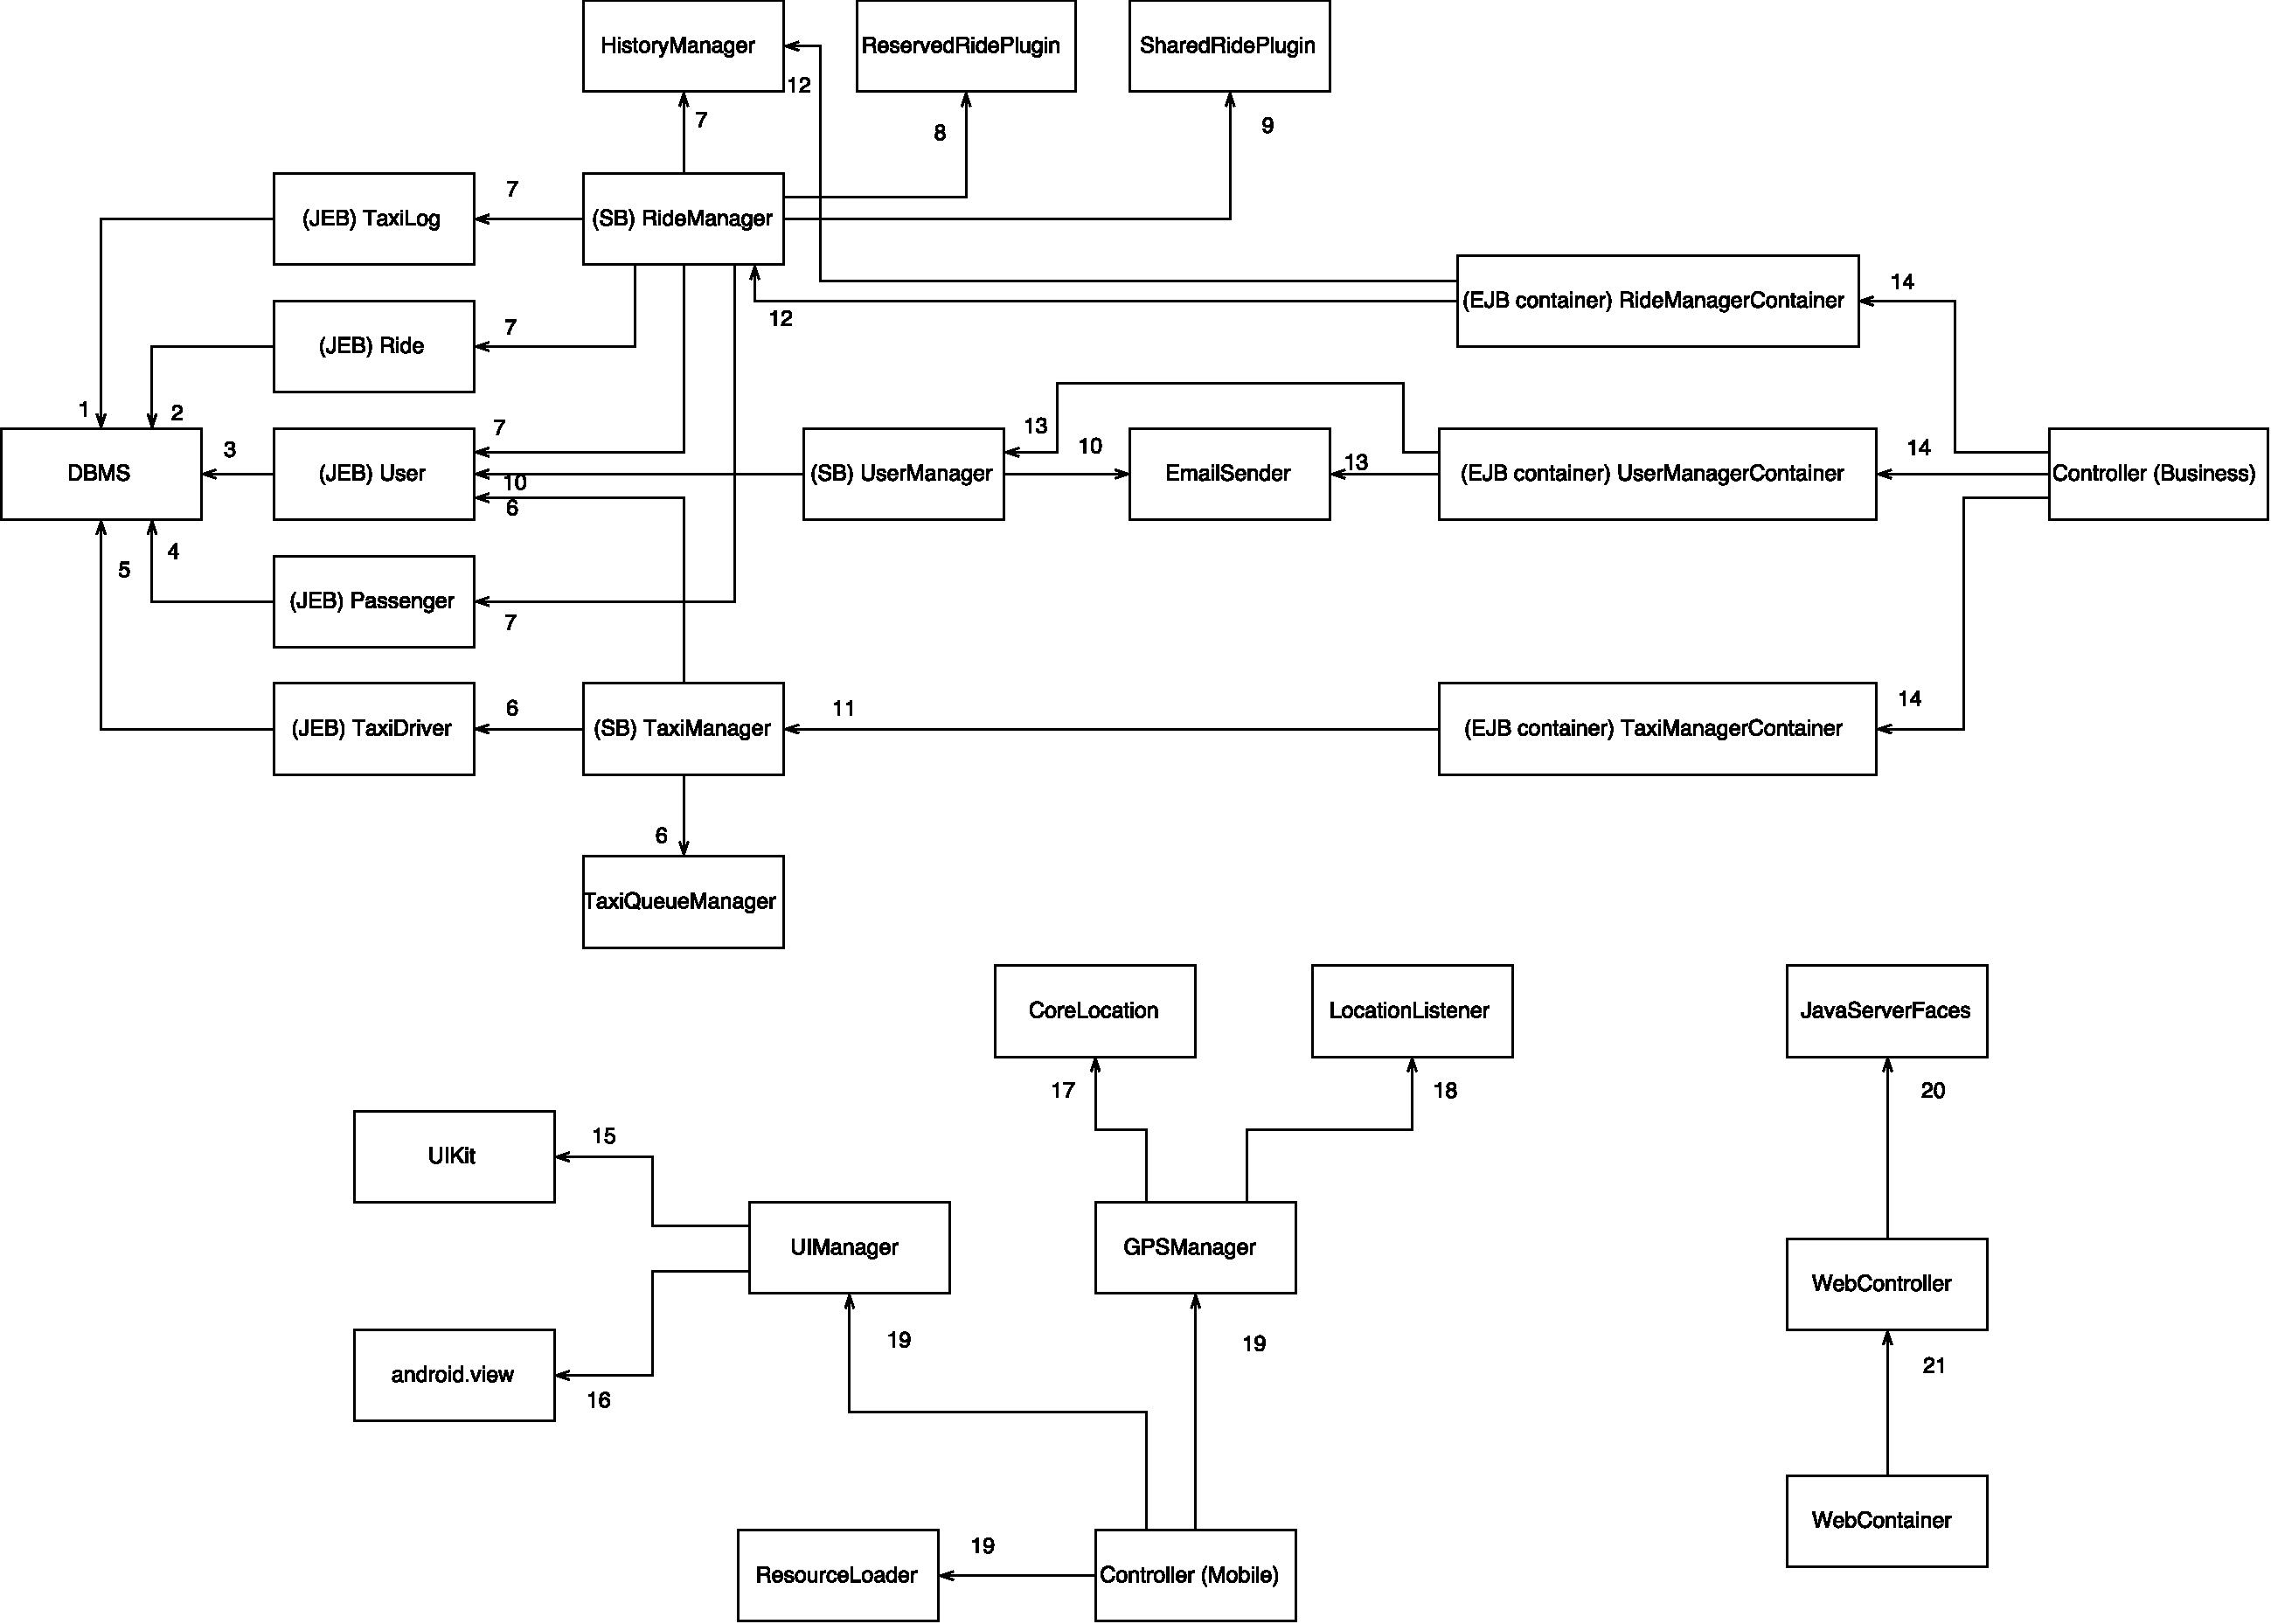
\includegraphics[width=\textwidth]{figures/components_integration.pdf}
    \caption{Diagram of the components integration.}
    \label{fig:components-integration}
\end{figure}

\subsection{Subsystem Integration Sequence}
The integration sequence of the subsystems is described in~\autoref{tab:subsystem-integration} and in~\autoref{fig:subsystem-integration}.

A choice was made to proceed with the integration process from the server side towards the client applications, integrating the mobile app before the web tier.
The reason to do so is that in order to have a functioning client you need to have a working business tier.
The business tier, instead, can be tested without any client, by making API calls also in an automated fashion.

By integrating the mobile application before the web tier, we aim to obtain a fully operational client-server system as soon as possible, since taxi drivers can not work without the mobile app.
The web tier is less essential and can be integrated after the app.

\begin{table}
    \centering
    \begin{tabular}{| l | l | l |}
        \hline
        \textbf{N.} & \textbf{Subsystem} & \textbf{Integrates with} \\
        \hline
        SI1 & Business tier & Database tier\\
        SI2 & Mobile application & Business tier\\
        SI3 & Web tier & Business tier\\
        SI4 & Client browser & Web tier\\
        \hline
    \end{tabular}
    \caption{Integration order of the subsystems described in~\autoref{sec:elements}.}
    \label{tab:subsystem-integration}
\end{table}

\begin{figure}
    \centering
    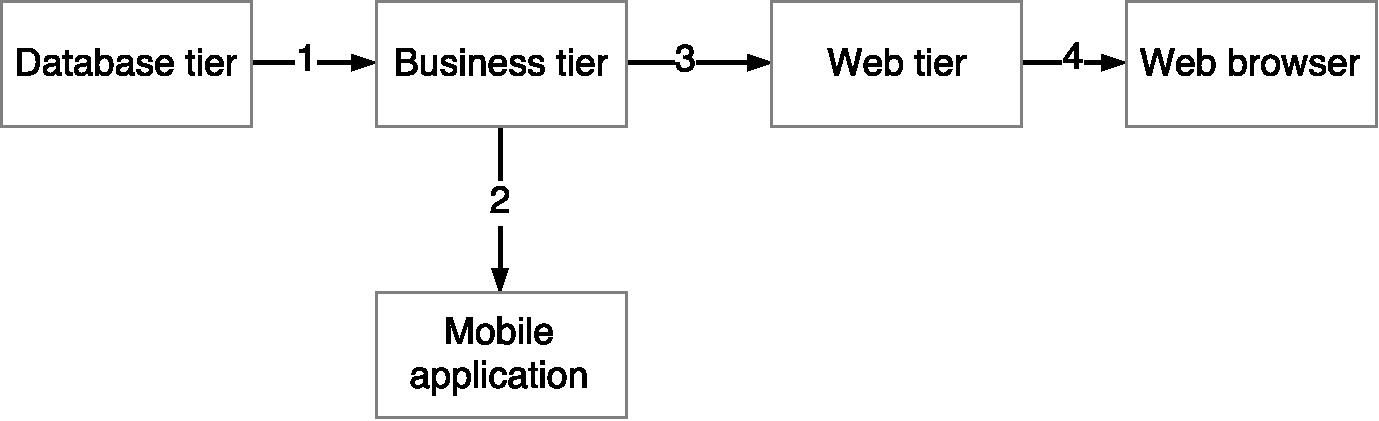
\includegraphics[width=\textwidth]{figures/subsystems_integration_dag.pdf}
    \caption{Directed Acyclic Graph representing the order of integration of the subsystems. See~\autoref{tab:subsystem-integration}.}
    \label{fig:subsystem-integration}
\end{figure}
